
%\documentclass[preprint,authoryear,12pt]{elsarticle}
\documentclass[times, 12pt,a4paper]{article}
\usepackage{graphicx,amssymb,amsthm,stmaryrd}%,booktabs}
\usepackage{times}
\usepackage{amsmath,url,algorithm,algorithmic,mathrsfs,makeidx}
\usepackage{graphicx}
\usepackage{epstopdf}
\usepackage{epsfig}
\usepackage{latex8}

%journal{Journal of Knowledge-Based Systems}



\begin{document}
%\begin{frontmatter}

\newtheorem{definition}{Definition}
\newtheorem{proposition}{Proposition}
\newtheorem{example}{Example}
\newtheorem{lemma}{Lemma}
\newtheorem{theorem}{Theorem}
\newtheorem{corollary} {Corollary}
\title{\underline{Response Letter}\\\vspace{0.5cm}Efficient Community Formation for Web Services}
\author{Ehsan Khosrowshahi Asl\\
e\_khosr@encs.concordia.ca\\
\and
Jamal Bentahar\\
bentahar@ciise.concordia.ca \\
\and
Hadi Otrok\\
hadi.otrok@kustar.ac.ae \\
\and
Rabeb Mizouni\\
rabeb.mizouni@kustar.ac.ae \\
}


\maketitle


First, we would like to thank and express our appreciation to the
reviewers for taking the time to carefully review our manuscript,
and for their insightful, valuable, and very useful comments. We
would like to thank the associate and chief editors as well for
their valuable comments and suggestions for improvements. We
carefully considered the comments and implemented all of them in
the revised version. In this letter, we will explain, point by
point, how the issues raised in the reviews are addressed and
answered. We hope our answers and revisions will satisfy the
reviewers and editors, which will make the paper accepted for
publication in IEEE Transactions on Services Computing (TSC).\\

%\newpage

%%%%%%%%%%%%%%%%%%%%%%%%% REVIEWER 1 %%%%%%%%%%%%%%%%%%%%%%%%%
\begin{center}
  \textbf{Reviewer 1}
\end{center}


\vspace{0.6cm} \textbf{\underline{Reviewer's appreciation}:} The
paper presents a nice modelling of community formation based on
coalition games. The authors defended well their approach and
provided good illustrative examples.

\vspace{0.2cm}\textbf{\underline{Answer}: Thank you for the
positive feedback.}


\vspace{0.5cm} \textbf{\underline{1. Reviewer}:} Page 4: Last
paragraph: should be $x_i$ instead of $i$ at the condition level.

\vspace{0.2cm}\textbf{\underline{Answer 1}: Thanks for the
comment. Actually, the confusion comes from Equation 2, which
should be $\forall S \subseteq N, \sum_{i \in S} x_i \geq v(S)$
instead of $\forall S \subseteq N, \sum_{x_i \in S} x_i \geq v(S)$
as $x_i$ is the payoff vector of the player $i$ and $S$ is the set
of all players. This has been fixed in Equation 2 and Equation 4
as well (Section 2.4).}

\vspace{0.5cm}\textbf{\underline{2. Reviewer}:}  Page 6: You
should relate $v(S)$ to $PO(C)$ in equations 5 and 6.

\vspace{0.2cm}\textbf{\underline{Answer 2}: The connection between
$v(S)$ and $PO(C)$ has been mentioned in Section 3.3, second
paragraph and when we described the algorithm of our scenario in
Section 4.1. To be more specific, the connection is between $v(C)$
and $Out(C)$ that is computed in Equation 6 based on $PO(C)$
computed in Equation 5. The connection is that the worth of a
community is set to the output the community can generate, i.e.,
$v(C) = Out(C)$. However, we agree that this should be reported
earlier. In the revised version it is clearly stated just after
Equation 6 (Section 3.2). }
% RABEB: I do not get what you mean by however we had .... I beleive taht you need to reformulate your answer by saying that : The connection between V(S) to PO(C) has been already defined when describing the algorithm of our scenario in section 4.1. To clarify it more, we modified the section and we added the connection at the end of the paragraph.



\vspace{0.5cm}\textbf{\underline{3. Reviewer}:} Page 7: Please add
some definitions such as the one for Grand coalition to make the
paper self-contained.

\vspace{0.2cm}\textbf{\underline{Answer 3}: In the revised
version, all the needed concepts are defined. Grand coalition is
defined as follows: In cooperative game theory, grand coalition is
a coalition that contains a maximum number of players as long as
they can maintain a stable (in terms of membership) and beneficial
(in terms of utility) group for all the players (Section 4.1,
paragraph 3).}


\vspace{0.5cm}\textbf{\underline{4. Reviewer}:} Why you didn't
leverage the foundations of repeated games instead of coalitional
games? Is there any strong reason?.

\vspace{0.2cm}\textbf{\underline{Answer 4}: The main objective of
this work is to optimize the gain of web service communities as a
whole and to ensure the creation of stable communities in terms of
joining and leaving activities. Such a problem is formulated by
the means of coalition games, a part of cooperative game theory
where the gain can be fairly distributed based on the contribution
of each member using the theory of \emph{shapley value}. In this
context, communities can be formed and have their stability
condition formulated based on the \emph{Core} solution concepts.
Repeated games fit better in situations where web services are
competing with each other so they can learn the best response by
playing the game repeatedly. In our case, web services are rather
cooperating where the objective of web services communities is to
motivate intra-community cooperation and to motivate quality web
services to join such communities. Because each community is seen
as a cooperative group where members cooperate to achieve a better
outcome, cooperative game theory methods provide us with great
decision mechanisms for forming groups and coalitions which would
benefit the agents involved altogether.}

\textbf{In fact, because members of the same community are
providing similar functionalities, one can argue that they are
competing with each other, rather than cooperating. However, the
main idea, and also the main innovation and contribution of the
paper is to show that those member web services can form strong
and stable communities as coalitions so that they can better
compete as a whole with other web services and other communities,
which will allow them to be better off. In other words, we are
promoting the idea of intra-community cooperation and
inter-community competition. This justifies the use of coalition
games instead of repeated games.}

\textbf{Because we found it important as motivation of our choice
of coalition games, this discussion is reflected in the revised
version in the introduction section (Section 1, Motivations part).
In this new part, we added examples from the business world to
highlight the cooperation strategy. This has been raised by
Reviewer 3 as well (see additional details in our Answer 1 to
Reviewer 3).}




%In repeated games, there should be a repeatable game between agents one to one. The  decision cannot be optimal for all the agents involved. We believe repeated game is more appropriate in cases where there is a lot of competing one-to-one interactions between agents  happening and not in coalitions.
 %and actually we are working on repeated games and specifically repeated game with learning techniques such as q-learning to help distribute the ``task distribution job'' among all the web services where web services are having different confidence states, and based on their action history and state they are in, web services can directly opt for getting and performing tasks alone or cooperating which other agents.
% RABEB: I do not see the need for the last sentence starting from and actually we are as you are opening the door for questioning our decision  ...



\vspace{0.5cm}\textbf{\underline{5. Reviewer}:} Page 8: What do
you mean by "the algorithm gets interrupted": is it based on a
logical condition? if yes, what is it?

\vspace{0.2cm}\textbf{\underline{Answer 5}: The interruption we
are mentioning can be either caused by time/memory constraints
when the number of subsets is big enough (timeout) or forced
manually by the system designer if for example the already
obtained results are satisfactory. In fact, if the algorithm gets
interrupted while verifying $depth(n)$, it will have $depth(n-1)$
already verified. Each depth will have $O(n^2)$ cases to check, so
for example if it reaches depth 10, and the algorithm gets
interrupted (manually or because of system resources), we at least
have checked for all the subsets of depth 9. Clarification has
been added in the revised manuscript at Section 4.1, last
paragraph.}


\vspace{0.5cm}\textbf{\underline{6. Reviewer}:} Page 9: Please
provide equations using $\lambda$ and $\epsilon$ and relate them
to your model that uses $R_C$.

\vspace{0.2cm}\textbf{\underline{Answer 6}: Thanks for this
suggestion. We added in the revised version the following equation
Equation 8 (Section 4.3, paragraph 2) linking the Shapley value of
a web service $i$ when moving from one community $C$ to another
one $C'$ to $\epsilon$.
%
\begin{equation*}\label{eq:gainsh}
g_i(C \rightarrow C') = \phi_i(C',v) - \phi_i(C,v) - \epsilon
\end{equation*}
%
It relates our model that uses $R_C$ and $\epsilon$ as the Shapley
value is computed using $v(C)$, which in turn is computed using
$Out(C)$ based on $R_C$. The idea is that before deciding to
change the community (from $C$ to $C'$), each web service $i$ has
to be sure that the gain $g_i(C \rightarrow C')$ calculated based
on the Shapley values of $i$ in the previous and new communities
and the tax $\epsilon$ is positive, which means, what the web
service would gain in $C'$ is greater than what it gains in $C$
and the tax it would pay if moving all together. Furthermore, we
added in paragraph 3 of the same section (Section 4.3) the
following linear program that determines the minimum value of
$\lambda$ that makes the community stable ($Core$ condition):
%
 \begin{alignat*}{3}
    \min~   & \lambda  \\
    \text{s.t. } & \lambda v(C) > v(C') & ~& \text{ for all } C' \subset C
  \end{alignat*}
%
}

\vspace{0.5cm}\textbf{\underline{7. Reviewer}:} Page 10: For the
$\epsilon$ core method: the value of $\epsilon$ should be varied
to verify its impact in the experiments section.

\vspace{0.2cm}\textbf{\underline{Answer 7}: Yes, the value of
$\epsilon$ should vary to verify its impact and that is exactly
what we are doing in our experiments. In the revised manuscript,
we changed the explanation to make this fact more clear: Section
5, paragraph 5. See also Fig. 5}

\vspace{0.5cm}\textbf{\underline{8. Reviewer}:} The experiments
are missing a comparison with [18].

\vspace{0.2cm}\textbf{\underline{Answer 8}: The experiment
illustrated in Figure 9 (Last paragraph of Section 5) presents a
comparison of our work with [18]. We have called their method
``High Availability Coalition model''. We highlight this in the
new caption of this figure.}

\vspace{0.5cm}\textbf{\underline{9. Reviewer}:} Scalability
evaluation is missing: what is the impact of increasing the number
of services/communities on the system efficiency?.

\vspace{0.2cm}\textbf{\underline{Answer 9}: We conducted
scalability tests. We used 10,000 communities consisting of 3 to
160 web services. This number is large enough since in the
concrete examples of coalitions in the airlines domain we are
implementing, the largest coalition, Star
Alliance\footnote{\url{www.staralliance.com}}, has 28 airline
members. When conducting our experiments using the real web
service data provided in
\url{http://www.uoguelph.ca/\textasciitilde{}qmahmoud/qws/}, in
average, the communities were populated by 60 web services. Thus,
in total, the number of used web services is 600,000. This makes
our system scalable enough. We also conducted experiments with a
large number of tasks from users up to 130 per iteration per
community, which means 6500 (130*50) tasks per community. We
observed that increasing the number of communities and web
services did not affect the overall efficiency of the system in
terms of coalition formation. In fact, as mentioned in the paper,
our algorithms run in $O(n)$ and $O(n^2)$ time as the number of
web services $(n)$ within a community grows. Thus, our algorithms
run in polynomial time. On the other hand, increasing the number
of tasks did not affect our results, since communities only accept
tasks at rate $R_C$. In the revised manuscript we highlighted the
runtime of our \emph{Depth-1 Convex-Checker} and \emph{Depth-2
Convex-Checker} methods in our experiments in Section 5, paragraph
4.}
%In case $R_C$ is set very large, communities can grow larger, and may suffer from  bottleneck due to huge number of task processing on a single server, a fact that is out of scope of this paper.


%%%%%%%%%%%%%%%%%%%%%%%%% REVIEWER 2 %%%%%%%%%%%%%%%%%%%%%%%%%
\vspace{2cm}

\newpage

\begin{center}
  \textbf{Reviewer 2}
\end{center}


\vspace{0.6cm} \textbf{\underline{Reviewer's appreciation}:} This
paper investigates into web services communities and the quality
of service in aggregating the web services in communities. The aim
is to maximize the efficiency through collaboration and through
forming coalitions of web services and improving the overall QoS
and revenue. The problem of web services community is interesting
as there exist a large number of web services with varying level
of QoS. The paper provides a good rationale behind the use and
establishment of communities of web services � esp. community web
services should be highly available and responsive; maintain
collaboration with others as well as maintain their own autonomy,
when used in business or any other settings.

The paper reviews the current work on web service communities and
QoS and identifies their strengths and weaknesses. It then
exploits the game theory approach and proposes a cooperative game
model for the aggregation of web services within communities. The
proposed model is well designed and developed. It�s also logically
mapped to the characteristics of web services they exhibit in
communities.

The proposed model is implemented as a prototype system and
various simulation experiments are conducted. The experimental
results show the benefits of the proposed model in terms of
stability, fairness, increase in revenue and in improvement of
user satisfaction.

Overall, the paper is well written and well structured.

\vspace{0.2cm}\textbf{\underline{Answer}: Thank you for the
positive feedback.}

\vspace{0.5cm}\textbf{\underline{1. Reviewer}:}  Though there's a
referral to [8] it'd be helpful to explain more the concept of
``Community coordinators'' web services, somewhere in the early
parts of the paper. How's it different from other (common) web
services in a given community?

``community master'' and ``community coordinator'' are these
different?

\vspace{0.2cm}\textbf{\underline{Answer 1}: First, there is no
difference between community master and community coordinator. To
avoid the confusion, we only use in the revised version the term
``community coordinator'' as community manager for our
architecture; ``community master'' has been kept only when it is
used as such in the literature. Second, we agree on your
suggestion and added the following explanation in Section 1,
paragraph 2: When communities are used, users send their requests
to the coordinators of those communities, which play the role of
their representatives or access points. Community coordinator is a
particular service that takes in charge the verification of
credentials of new web services before accepting them to join the
community, inviting good web services to join the community,
firing bad web services if they don't perform as expected, etc.
The coordinator is responsible for all the operations related to
the management of the community infrastructure in terms of
regulating the membership and insuring that the overall
performance is satisfactory. Unlike web services that are members
of the community, the coordinator does not offer services directly
to the users, it only forwards the requests to the suitable
members. The coordinator is created by the community owner when
the community is initiated.}

\vspace{0.5cm} \textbf{\underline{2. Reviewer}}: p.4 ``If he is
added to the set $S$,�'', ``his contribution�'' not sure `he' and
`his' are the right terminologies.

\vspace{0.2cm}\textbf{\underline{Answer 2}: We agree, we rephrased
the sentence as follows:  If the member $i$ is added to the set
$S$, the contribution of this set to the coalition is $v(S \cup
\left\{i\right\}) - v(S)$.}

\vspace{0.5cm} \textbf{\underline{3. Reviewer}}: p.10 ``our
community receives 130 tasks from users'' what are the types of
tasks. Are these simulated or real functions that need to
performed by web services?

\vspace{0.2cm}\textbf{\underline{Answer 3}: In the previous
version, the tasks were abstract. In the revised version, the
tasks are real tasks about flight booking that need to be
performed by web services. The users provide the flight dates, the
origin and destination, type of tickets, and number of guests. Web
services will find different flights with different companies,
prices, timing, etc. During our experiments, the tasks are
randomly generated and are coded as XML requests (String) and
responses are also coded in XML. Based on community task queue
delay and the assigned web service quality metrics (such as
reliability, throughput, latency and other metrics) these tasks
will be performed with different qualities. In the experimental
results and analysis section (Section 5), we have illustrated and
evaluated the average QoS of tasks performed. In the revised
manuscript, we added more explanations and details about the tasks
in Section 5. Other details are also mentioned in our Answer 5 to
Reviewer 3.}


\vspace{0.5cm} \textbf{\underline{4. Reviewer}}: p.9 �agents would
only earn a minimal amount of e by deviating�.� �by deviating from
what?

\vspace{0.2cm}\textbf{\underline{Answer 4}: We mean deviating from
the coalition. This has been fixed in the revised version.}



%%%%%%%%%%%%%%%%%%%%%%%%% REVIEWER 3 %%%%%%%%%%%%%%%%%%%%%%%%%
\vspace{2cm}

\newpage

\begin{center}
  \textbf{Reviewer 3}
\end{center}

\vspace{0.6cm}\textbf{\underline{1. Reviewer}:}  It is not
convincing that the formation of service community can be modeled
as a cooperative gaming problem.


\vspace{0.2cm}\textbf{\underline{Answer 1}: As argued in our
Answer 2 to Reviewer 1, we are advocating the idea of community as
a way to group web services in order to increase the total gain of
all the members where each web service gain is more than or equal
to what this web service would obtain being outside the community.
This is because the community can provide wider visibility, better
market share, higher reputation, and better way of sharing
resources. Community for us is an infrastructure and being part of
it should benefit the web service, but also the community as a
whole. As argued in [Maamar et al., 2011]\footnote{Z. Maamar, P.
Thiran, and J. Bentahar (2011). Web services communities: from
intra-community Coopetition to inter-community Competition. In
E-Business Application for Product Development and Competitive
Growth: Emerging Technologies, In Lee editor, pp. 333-343, IGI
Global.}, inside a community, web services can either compete or
cooperate. In this paper, we stress the intra-community
cooperation between web services for a better inter-community
competition. The main idea is that to form a stable web service
community and to have fair distribution of the total gain based on
the contribution of each individual, cooperative game theory,
particularly coalition game theory, is very suitable to formalize
such a problem. Cooperation between competitors is a well
established practice in economical theories (see for instance
[Chetty and Wilson 2003]\footnote{S. K. Chetty and H. I. M. Wilson
(2003). Collaborating with competitors to acquire resources.
International Business Review, vol. 12. pp. 61-81.} and [Bucklin
and Sengupta 1993]\footnote{L. P. Bucklin and S. Sengupta (1993).
Organizing successful co-marketing alliances. Journal of
Marketing. vol. 57, pp. 32-46.}). This happens in real business
world scenarios. As an example, let us consider major carrier
airlines providing ticket selling services. Those airlines can be
seen as competing agents, each one tries to maximize its utility
by gaining more market share. However, nowadays those companies
are usually part of different coalitions (alliances) such as Star
Alliance\footnote{\url{www.staralliance.com}} (28 airline members
including Scandinavian Airlines, Thai Airways International, Air
Canada, Lufthansa, and United Airlines),
SkyTeam\footnote{\url{www.skyteam.com}} (19 members, among them
Aerom\'{e}xico, Air France, Delta Air Lines, Continental Airlines,
KLM, and Northwest Airlines), and Oneworld\footnote{\url{
www.oneworld.com}} (13 members including Air Berlin, American
Airlines, British Airways, Cathay Pacific, Iberia, Japan Airlines,
Malaysia Airlines, and Qatar Airways). By sharing resources and
market share and having the option of service multi-hop air
tickets combined from different airlines, each airline member of a
coalition can increase its gain by collaborating. The question is
when this collaboration would be beneficial for all the agents
involved? For example the three alliances would not gain anything
by collaborating and sharing resources with airlines of low
reputation and quality. They will lose their market and would
rather stay away from this collaboration. Therefore, no stable
community can be formed between well established and poor
airlines. Another example of cooperation among competitors is the
arrangement between PSA Peugeot Citro\"{e}n and Toyota to create
Toyota Peugeot Citro\"{e}n Automobile
(TPCA)\footnote{\url{www.tpca.cz/en/}} in order to share
components for a new city car where the different companies save
money on shared costs while remaining competitive in other areas.
Our solution of cooperation between competitor web services within
coalitions follows these models. We updated the paper to reflect
this important discussion by adding a new part, called
motivations, to the introduction (Section 1).}


\vspace{0.5cm}\textbf{\underline{2. Reviewer}:}  First, the
concept of service community used in this paper is different from
the ones used in the existing work, such as in the referred
papers. The general idea of service community is a homogeneous
service group that conceptually include services providing similar
functionality. Services in the same community are independent and
autonomous. There is no central control mechanism for the
community. On the other hand, the concept of service community of
this paper is a group of services which are monitored and managed
by a community manager. It is not clear how realistic or practical
such a community is and what the real world examples are.


\vspace{0.2cm}\textbf{\underline{Answer 2}: Most of the existing
work have clearly stated that communities of web services need a
centralized manager for the purposes of developing, coordinating
and managing the community infrastructure and in some of the
works, being the access point of the community and having the role
of delegating tasks:
%
\begin{itemize}
%
\item {[Liu et al. 2012][28]} (published in the same journal IEEE
Transactions on Services Computing, 2012): The authors used a very
similar architecture to the one we are using in our paper. Each
web service community has a \emph{coordinator} which is
responsible for receiving and satisfying customers' requests and
``\underline{managing the cooperation among the members}''. The
coordinator plays then the role of the community manager.
%
\item {[Lim et al. 2012][26]}: The paper uses exactly the
architecture we are using here. Each community is managed by a
\emph{Master Web Service}.
%
\item {[Benatallah et al. 2003][9]}: The paper introduces the
concept of \emph{service container}, which plays the role of
community and its manager at the same time.  A container is a
service that aggregates several functionally similar services.
Containers exist independently of the services they aggregate. The
service container is the one to invoke instead of an elementary or
composite service aggregated by that container.
%
\item {[Maamar et al. 2008][14], [Maamar et al. 2009][8]}: Here
again the architecture proposed in these papers is the one we are
using in our work.
%
\item {[Zeng et al. 2003][11]}: The paper describes a global
planning selection algorithm and a delegation algorithm to be run
when a request to execute an operation is received by the
community. This needs a central entity to run those algorithms.
Such entity plays the role of the community coordinator or
manager.
%
\item {[Medjahed and Bouguettaya 2005][13]}: The paper describes
the concept of \emph{community agents} associated to
\emph{community providers}. A community agent is responsible,
among other things, of the registration of services with the
community. The paper uses the example of a community that provides
health care services to senior citizens. In this example, a
governmental entity is needed to check the health care standards
used by the members before authorizing them to be part of the
community. Such a central entity is represented by the community
agent. Thus, community agents are playing the role of community
managers.
%
\item {[Limam and Akaichi 2010]}\footnote{H. Limam and J. Akaich.
Managing web services communities: A cache for queries
optimisation, International Journal on Web Service Computing,
Vol.1, No.1, pp 2230-7702, 2010}: The paper describes explicitly
the concept of \emph{centralized access} in the community
definition.
%
\end{itemize}
%
It is worth mentioning that in our work, service community is also
a homogeneous service group that hosts services providing similar
functionalities. Moreover, services in the same community are also
independent and autonomous in our work. They are self-interest and
utility maximizer agents, and behave autonomously towards
maximizing their own profits using our game theory approach. They
have the freedom to leave the community anytime if they are not
satisfied about the profit they are making. Having a community
manager, only means that the management of the community
infrastructure in terms of accepting new web services and
verifying the credentials of the members is centralized. In other
words, the coordinator does not manage web services, but does
manage the community. The manager does not dictate what the web
services should do and how they should behave. In fact, all the
existing proposals agree that because the community is an
infrastructure that hosts different web services, membership
cannot be leaved open so that any web service can join even those
having poor quality and bad reputation. A community is a system
that should accept only particular web services, and there should
be a mechanism to control the credentials of the members.}

\textbf{Going back to the real world example of airlines
alliances:
%
\begin{itemize}
%
\item Star Alliance is managed by a centralized company \emph{Star
Alliance Services GmbH}, which was created on behalf of its
members and led by the current CEO, Mark Schwab. Star Alliance
Services GmbH is responsible of coordinating the development and
strategies of the airline alliance from its base in Frankfurt am
Main,
Germany\footnote{\url{www.staralliance.com/en/about/organisation/}}.
%
\item SkyTeam has centralized core management team, \emph{SkyTeam
Central}, based at the World Trade Center Schiphol Airport and led
by the current Chairman of the SkyTeam Governing Board, Leo van
Wijk. The core management team ``is responsible for overseeing
day-to-day operations of the alliance, including: marketing,
sales, airport synergies and transfer product, cargo, advertising
and brand, alliance operations, finance, corporate communications
and alliance
administration''\footnote{\url{http://www.skyteam.com/en/About-us/Organization/Management/}}.
%
\item Oneworld is managed by its central alliance office, the
\emph{Oneworld Management Company} (\emph{oMC}) based in New York
City and led by Tom Horton (Chairman) and Bruce Ashby (CEO). The
oMC acts as the alliance's central secretariat, with
responsibility for driving future growth and the launch of new
customer services and
benefits\footnote{\url{www.oneworld.com/news-information/oneworld-fact-sheets}}.
%
\end{itemize}
%
In all these alliances, accepting a new member or pending a member
is decided centrally. Regarding the second example, TPCA coalition
is also managed by a central management company based in the
industrial zone of Kolin - Ov\v{c}\'{a}ry, Czech republic and led
by Kenta Koide,
president\footnote{\url{www.tpca.cz/en/about-us/management-tpca-en-us/}}.}
%

\textbf{In the revised manuscript, we reported these discussions
in the motivation part of the introduction (Section 1) and in the
related work section (Section 2).}


\vspace{0.5cm}\textbf{\underline{3. Reviewer}:}  The problem is
modeled in a way so that the cooperative game theory can be
applied, but not in a way that is consistent with the real world
scenarios.

\vspace{0.2cm}\textbf{\underline{Answer 3}: Answers 1 and 2 are
answers for this comment as well.}

\vspace{0.5cm}\textbf{\underline{4. Reviewer}:}  The service
parameters, such as its request rate and  throughput rate are not
in line with the general characteristics of web services, such as
input and output parameters. It is not clear how the proposed
service parameters are obtained and why they are important to
determine a service's membership to a community, considering that
they depend on not only the service's capacity, but also the
amount and frequency of user requests, which can be random.


\vspace{0.2cm}\textbf{\underline{Answer 4}: First, we have to
mention that we are focusing on \underline{quality metrics}, which
are non-functional. Our proposal is general and independent from
the functional input-output parameters. The parameters we are
using are the typical parameters of web services,  which are
obtained from a real world data set provided at:
\url{http://www.uoguelph.ca/\textasciitilde{}qmahmoud/qws/}. The
request rate was inspired by market share and reputation models of
communities of web services, which have been used in other
proposals such as [17],[23]. Those parameters are important as
community coordinators tend to accept only good web services which
provide good QoS and have the potential to increase the utility of
the community. It has been showed in [23] that the request rate is
positively correlated with the trust and performance of web
services, which means it is not random when the service is running
for a large enough period of time. In fact, having a
\emph{casi-static} request rate for communities is not
unrealistic. To support our claim, we provide data from a real
world example. The CEO of \url{concertboom.com}, Kooshiar Azimian,
has provided us with their access and request rates of the web
services they use\ref{cblog}. Their service provides ticketing
information for events happening close to user's location. They
use Ticketnetwork.com web services\footnote{Affiliate program
link: http://www.ticketnetwork.com/affiliates/agreement.aspx}
\footnote{Web Service API documentation:
\url{www.getacoder.com/data/projects/77613/TicketNetwork\%20Web\%20Services\%20(W2)-.doc}},
and have implemented their back-end code in Java. As shown in
Figure \ref{fig1}, they currently have an average of 340,000 daily
page views or almost 3.95 requests per second. They invoke the
\url{ticketnetwork} web service almost 4 times per second to get
the seating chart and tickets available for the events. During a
day, the pick time happens at around 20:00 UTC time, which has
almost 10\% more requests than during the lower pick time, which
happens around 7:00 AM UTC time. As shown in the figure, the
pattern of request rate is casi-stable during the period between
May and September.
%Therefore, \url{ticketnetwork} knows that
%\url{concertboom.com} has a request rate of 340,000 requests per
%day or almost 3.95 requests per second and can adjust the internal
%service providers and resources so they can  provide these rate of
%services.
}

\textbf{Because the data of \url{concertboom.com} are private, we
were asked not to disclose them publicly. We only get from the
company the consensus to use them for the response letter. This is
the reason why we could not add them to the paper.}

\begin{figure}
\begin{center}
%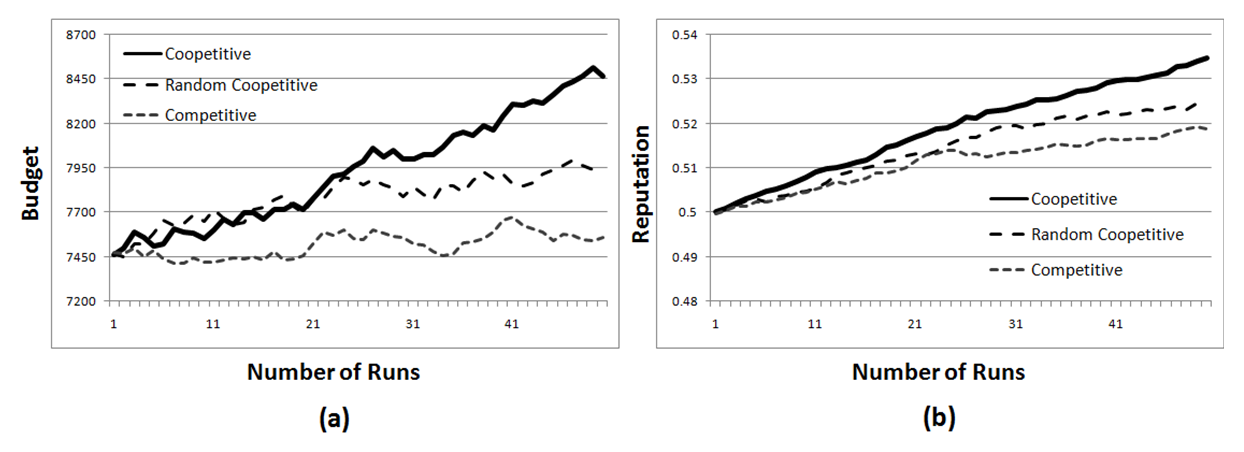
\includegraphics[scale=0.6]{graph1Final+.eps}
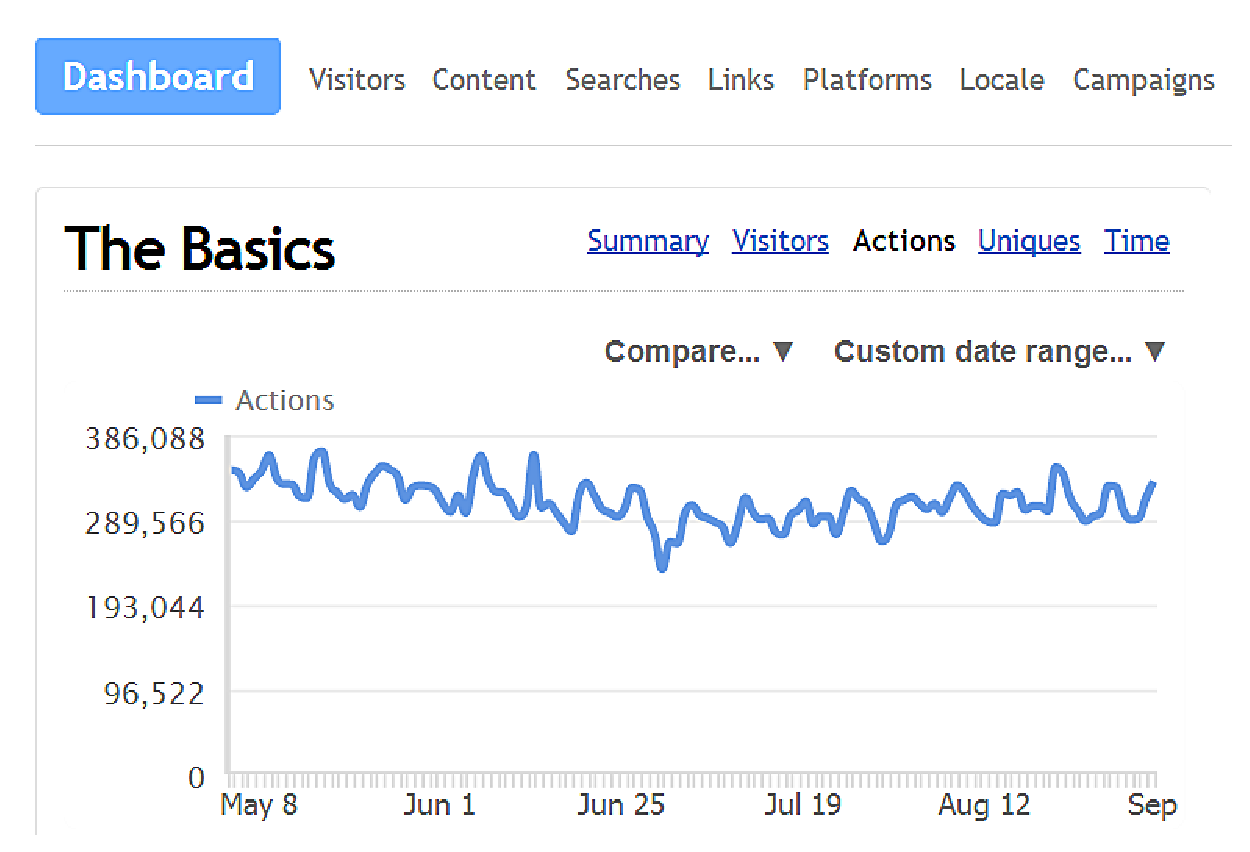
\includegraphics[width=10cm]{cb.eps}\label{cblog}
\caption{Number of ticket pageviews of concertboom.com during May 5th, until Sep 9th, 2013}
\label{fig1}
\end{center}
\end{figure}

\vspace{0.5cm}\textbf{\underline{5. Reviewer}:}  The paper
conducted a simulation instead of an experimental study using real
world web services. This also suggests the difficulties of finding
real world examples and application for the proposed idea.


\vspace{0.2cm}\textbf{\underline{Answer 5}:
%Our focus is on non-functional properties of web services and is extendable to any type of web service communities providing any type of service, which there is high demand, request load and competition for that service type such as mapping, weather, ticketing, and local places information.
As mentioned previously, for our experiments, we have implemented
our web services using real data extracted from a data set of web
services
(\url{http://www.uoguelph.ca/\textasciitilde{}qmahmoud/qws/}).
This makes our web services behave like real ones. In the previous
version, web services were implemented as abstract enteties as the
main purpose was to focus on the quality metrics. In the revised
version, we use flight booking services and airlines coalitions as
concrete application domain. An XML SOAP based messaging system is
also implemented. The request contains the flight dates, the
origin and destination, type of tickets, and number of guests. The
response contains different flights with different companies,
prices, timing, etc. We have gathered around 200,000 flights and
stored them in our MongoDB database. As expected, this did not
affect our experimental results, since our concern, as most of the
related work, is on non-functional properties of web services. We
could deploy web services using JAX-WS in Java and deploy on
different servers. However, those web services would not reflect
the quality of service parameters of real web services under load
in real world. For example, we cannot evaluate the exact
bottlenecks different type of services may have, some qualities
may drop because of heavy load of DB queries, some because of
network congestions and delays while trying to generate the
results for end users. Therefore, the real world data can provide
us with QoS values of real functioning web services online. We
have carefully examined many published proposals in services
computing including work on web service community and composition
such as [Yu 2013]\footnote{Q. Yu and A. Bouguettaya, Efficient
Service Skyline Computation for Composite Service Selection, IEEE
Transactions on Knowledge and Data Engineering (TKDE), vo. 25, no.
4, pp. 776-789, 2013}, [Limam 2010]\footnote{H. Limam and J.
Akaich. Managing web services communities: A cache for queries
optimisation, International Journal on Web Service Computing,
Vol.1, No.1, pp 2230-7702, 2010}, [Liu 2012]\footnote{A. Liu, Q.
Li, L. Huang, S. Ying, and M. Xiao,Coalitional game for
community-based autonomous web services cooperation, IEEE
Transactions on Services Computing, vol. 99, no. PrePrints, 2012.}
and many others; we found that they evaluated their results using
a similar methodology. For the real world applications part of the
comment, see the previous answers.}




\vspace{0.5cm}

\vspace{1cm}








{
%\bibliographystyle{plain}
%\bibliography{omar}
}
\end{document}
